\chapter{Arhitektura i dizajn sustava}
		
		\textbf{\textit{dio 1. revizije}}\\
		
		
		Arhitektura ovog sustava je bazirana na arhitekturi klijent-poslužitelj. Sustav se sastoji od 3 sloja: sloj korisničkog sučelja, sloj aplikacijske logike, sloj podataka.
		
		Korisnik koristi aplikaciju preko web preglednika. Web preglednik je program koji omogućuje klijentu komunikaciju s web poslužiteljem aplikacije. Preglednik nam omogućava prikaz sloja korisničkog sučelja sustava. Korisnik preko web preglednika komunicira s web poslužiteljem slanjem i primanjem HTTP zahtjeva. Primljene podatke i datoteke web preglednik zna interpretirati i prikazati korisniku tako da sama interakcija s aplikacijom bude jednostavna.
		
		Web poslužitelj je računalo na kojem se aplikacija pokreće. Na njemu se dakle nalazi sloj aplikacijske logike. Web poslužitelj aplikaciji prosljeđuje zahtjeve na obradu i njezine odgovore prosljeđuje natrag klijentima. Web aplikacija na poslužitelju obrađuje zaprimljene zahtjeve. Ako obrada zahtjeva to zahtjeva, web aplikacija dodatno komunicira sa slojem podataka.
		
		Sloj podataka je predstavljen bazom podataka. U bazi podataka se na siguran način spremaju svi podaci koje je potrebno trajno čuvati. To podrazumijeva podatke o prijavama, korisničkim računima i slično. Takvi podaci moraju ostati očuvani i ako je rad aplikacije prekinut iz bilo kojeg razloga. Baza podataka je detaljnije opisana u poglavlju  4.1.
		
		Web aplikacija je podijeljena na frontend i backend.
		
		Frontend je zapravo prezentacijski dio aplikacije. On zapravo oblikuje korisničko sučelje i samim time definira što će korisnik vidjeti na web pregledniku kada koristi aplikaciju.
		
		Backend je dio aplikacije koji obrađuje zahtjeve i kontrolira rad ostalih dijelova sustava.
		
		Arhitektura same web aplikacije je odrađena u stilu MVC arhitekture. U ovoj arhitekturi aplikacija se dijeli na 3 sloja, svaki sa svojom ulogom. Ovime se postiže podjela odgovornosti pojedinih komponenti sustava. Sama struktura aplikacije je preglednija i smislenije primjenom ove arhitekture. Također, razvoj i održavanje sustava je znatno olakšan primjenom ove arhitekture. MVC arhitektura je izuzetno popularna u razvoju web aplikacija te je stoga dobro razrađena i mnogi radni okviri podržavaju njezinu implementaciju. MVC arhitekura se sastoji od slojeva:
		\begin{packed_item}
			\item \textbf{Model} - predstavlja komponentu aplikacije koja modelira aplikacijsku logiku. Ovaj model preslikava podatke dobivene od korisnika u bazu podataka i obrnuto. Na temelju zaprimljenih podataka vrši obradu zahtjeva.
			
			\item \textbf{Pogled(View)} - predstavlja dio aplikacije zadužen az prikaz podataka korisniku. Također omogućava korisniku interakciju s aplikacijom kroz prikaz korisničkog sučelja. Usko je povezan s frontend dijelom aplikacije.
			
			\item \textbf{Upravljač(Controller)} - upravlja nadolazećim zahtjevima. Ova komponenta prosljeđuje zahtjeve modelu na obradu. Od modela zaprima odgovore koje prosljeđuje komponenti za pogled na formiranje grafičkog prikaza koje se zatim prikazuje korisniku.
		\end{packed_item}
		
		Kroz međusobnu interakciju ova 3 modela omogućuju normalno funkcioniranje aplikacije.
		
		\begin{figure}[H]
			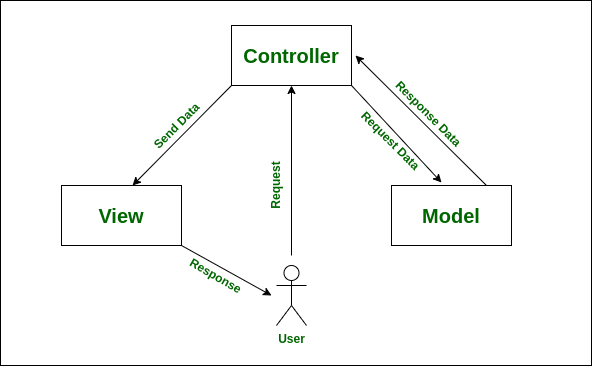
\includegraphics[width=\textwidth]{slike/mvc.png} %veličina u odnosu na širinu linije
			\caption{prikaz komponenti u MVC arhitekturi}
			\label{fig:MVC1} %label mora biti drugaciji za svaku sliku
		\end{figure}
		
		Za razvoj frontend dijela aplikacije odlučili smo koristiti programski jezik JavaScript uz radni okvir React. Backend dio aplikacije je realiziran u programskom jeziku Java uz radni okvir Spring Boot.
		

		\textit{ Potrebno je opisati stil arhitekture te identificirati: podsustave, preslikavanje na radnu platformu, spremišta podataka, mrežne protokole, globalni upravljački tok i sklopovsko-programske zahtjeve. Po točkama razraditi i popratiti odgovarajućim skicama:}
	\begin{itemize}
		\item 	\textit{izbor arhitekture temeljem principa oblikovanja pokazanih na predavanjima (objasniti zašto ste baš odabrali takvu arhitekturu)}
		\item 	\textit{organizaciju sustava s najviše razine apstrakcije (npr. klijent-poslužitelj, baza podataka, datotečni sustav, grafičko sučelje)}
		\item 	\textit{organizaciju aplikacije (npr. slojevi frontend i backend, MVC arhitektura) }		
	\end{itemize}
	\eject
	
		

		\section{Baza podataka}
			
			\textbf{\textit{dio 1. revizije}}\\
			
		\textit{Potrebno je opisati koju vrstu i implementaciju baze podataka ste odabrali, glavne komponente od kojih se sastoji i slično.}
		
			\subsection{Opis tablica}
			

				\textit{Svaku tablicu je potrebno opisati po zadanom predlošku. Lijevo se nalazi točno ime varijable u bazi podataka, u sredini se nalazi tip podataka, a desno se nalazi opis varijable. Svjetlozelenom bojom označite primarni ključ. Svjetlo plavom označite strani ključ}
				
				
				\begin{longtblr}[
					label=none,
					entry=none
					]{
						width = \textwidth,
						colspec={|X[6,l]|X[6, l]|X[20, l]|}, 
						rowhead = 1,
					} %definicija širine tablice, širine stupaca, poravnanje i broja redaka naslova tablice
					\hline \SetCell[c=3]{c}{\textbf{korisnik - ime tablice}}	 \\ \hline[3pt]
					\SetCell{LightGreen}IDKorisnik & INT	&  	Lorem ipsum dolor sit amet, consectetur adipiscing elit, sed do eiusmod  	\\ \hline
					korisnickoIme	& VARCHAR &   	\\ \hline 
					email & VARCHAR &   \\ \hline 
					ime & VARCHAR	&  		\\ \hline 
					\SetCell{LightBlue} primjer	& VARCHAR &   	\\ \hline 
				\end{longtblr}
				
				
			
			\subsection{Dijagram baze podataka}
				\textit{ U ovom potpoglavlju potrebno je umetnuti dijagram baze podataka. Primarni i strani ključevi moraju biti označeni, a tablice povezane. Bazu podataka je potrebno normalizirati. Podsjetite se kolegija "Baze podataka".}
			
			\eject
			
			
		\section{Dijagram razreda}
		
			\textit{Potrebno je priložiti dijagram razreda s pripadajućim opisom. Zbog preglednosti je moguće dijagram razlomiti na više njih, ali moraju biti grupirani prema sličnim razinama apstrakcije i srodnim funkcionalnostima.}\\
			
			\textbf{\textit{dio 1. revizije}}\\
			
			\textit{Prilikom prve predaje projekta, potrebno je priložiti potpuno razrađen dijagram razreda vezan uz \textbf{generičku funkcionalnost} sustava. Ostale funkcionalnosti trebaju biti idejno razrađene u dijagramu sa sljedećim komponentama: nazivi razreda, nazivi metoda i vrste pristupa metodama (npr. javni, zaštićeni), nazivi atributa razreda, veze i odnosi između razreda.}\\
			
			\textbf{\textit{dio 2. revizije}}\\			
			
			\textit{Prilikom druge predaje projekta dijagram razreda i opisi moraju odgovarati stvarnom stanju implementacije}
			
			
			
			\eject
		
		\section{Dijagram stanja}
			
			
			\textbf{\textit{dio 2. revizije}}\\
			
			\textit{Potrebno je priložiti dijagram stanja i opisati ga. Dovoljan je jedan dijagram stanja koji prikazuje \textbf{značajan dio funkcionalnosti} sustava. Na primjer, stanja korisničkog sučelja i tijek korištenja neke ključne funkcionalnosti jesu značajan dio sustava, a registracija i prijava nisu. }
			
			
			\eject 
		
		\section{Dijagram aktivnosti}
			
			\textbf{\textit{dio 2. revizije}}\\
			
			 \textit{Potrebno je priložiti dijagram aktivnosti s pripadajućim opisom. Dijagram aktivnosti treba prikazivati značajan dio sustava.}
			
			\eject
		\section{Dijagram komponenti}
		
			\textbf{\textit{dio 2. revizije}}\\
		
			 \textit{Potrebno je priložiti dijagram komponenti s pripadajućim opisom. Dijagram komponenti treba prikazivati strukturu cijele aplikacije.}